\section{Result Analysis and Discussion}
\label{sec:results}
From Table \ref{tab:results}, it should be confirmed that finding solutions to deal with the data shortage is critical. Indeed, the CNN downgrades significantly when we reduce the amount of training data from 100\% to 25\%. Specifically, the AUC of CNN decreases 5\%, 9\%, \%6, and 2\% on FLOW016, MNMX, SUBINC, and SUMTRIAN, respectively. This issue also happens in the cases of Accuracy and F1. Unlikely, transferable models work more stable with less data. Taking the 25\% data as an example, the pretraining the autoencoder in the multitask model (AE\_CNN\_Mul) achieves the highest performance on all the datasets.             

In terms of dealing with limited data, our proposed models outperforms transfer learning.  

Less sensitive

Considering the ability to distinguish among faulty types, 

Good representation



...Fig. \ref{fig:auc} shows ... Fig. \ref{fig:visualize} shows...

\begin{table*}[ht]
\centering
\caption{The comparison of the methods according to Accuracy, F1, and AUC. Each row block shows the classification performance for the use of 100\%, 75\%, 50\%, and 25\% of labelled training data. Each cell is in the form of mean $\pm$ standard deviation for 5 times of running.}
\label{tab:results}
\begin{adjustbox}{width=\textwidth}
% Please add the following required packages to your document preamble:
% \usepackage{multirow}
\begin{tabular}{lcccccccccccc}
\hline
\multirow{2}{*}{Approach} & \multicolumn{3}{c}{FLOW016}                                    & \multicolumn{3}{c}{MNMX}                                       & \multicolumn{3}{c}{SUBINC}                                     & \multicolumn{3}{c}{SUMTRIAN}                                   \\ \cline{2-13} 
                          & Acc.                & F1                  & AUC                & Acc.                & F1                  & AUC                & Acc.                & F1                  & AUC                & Acc.                & F1                  & AUC                \\ \hline
\textbf{100}&&&&&&&&&&&& \\
CNN                  & 72.52$\pm$0.23          & 71.34$\pm$0.15          & 0.80$\pm$0.08          & 81.99$\pm$0.06          & 80.03$\pm$0.21          & 0.80$\pm$0.02          & 70.93$\pm$0.71          & 69.94$\pm$0.32          & 0.72$\pm$0.11          & 67.97$\pm$0.34          & 66.35$\pm$0.42          & 0.77$\pm$0.19          \\
CNN\_Trans        & 73.05$\pm$0.54          & 71.67$\pm$0.43          & 0.81$\pm$0.34          & 81.53$\pm$0.31          & 79.07$\pm$0.55          & 0.80$\pm$0.11          & 69.08$\pm$0.92          & 68.15$\pm$0.81          & 0.74$\pm$0.52          & 67.12$\pm$0.73          & 66.06$\pm$0.56          & 0.79$\pm$0.11          \\
AE\_CNN              & \textbf{74.83$\pm$0.25} & 72.92$\pm$0.21          & 0.81$\pm$0.10          & \textbf{83.43$\pm$0.31} & \textbf{81.44$\pm$0.37} & \textbf{0.81$\pm$0.28} & 72.59$\pm$0.66          & \textbf{71.62$\pm$0.28} & 0.73$\pm$0.38          & \textbf{68.09$\pm$0.87} & \textbf{67.33$\pm$0.51} & 0.78$\pm$0.21 \\
CNN\_Mul       & 73.90$\pm$0.32          & 72.55$\pm$0.33          & 0.80$\pm$0.12          & 82.11$\pm$0.29          & 81.05$\pm$0.08          & 0.80$\pm$0.12          & 71.47$\pm$0.82          & 70.32$\pm$0.41          & 0.73$\pm$0.41          & 66.66$\pm$0.63          & 65.69$\pm$0.66          & 0.78$\pm$0.58          \\
AE\_CNN\_Mul   & 73.96$\pm$0.18          & \textbf{73.06$\pm$0.11} & \textbf{0.82$\pm$0.07} & 83.06$\pm$0.23          & 81.12$\pm$0.10          & 0.80$\pm$0.03          & \textbf{72.63$\pm$0.59} & 71.40$\pm$0.25          & \textbf{0.74$\pm$0.22} & 67.53$\pm$0.81          & 66.54$\pm$0.47          & \textbf{0.79$\pm$0.17} \\ \hline
\textbf{75}&&&&&&&&&&&& \\
CNN                   & 71.95$\pm$0.33          & 70.40$\pm$0.31          & 0.78$\pm$0.53          & 79.96$\pm$0.23          & 78.62$\pm$0.73          & 0.78$\pm$0.70          & 70.62$\pm$0.55          & 69.99$\pm$0.52          & 0.72$\pm$0.11          & 65.99$\pm$0.48          & 64.9$\pm$0.33           & 0.78$\pm$0.22          \\
CNN\_Trans         & 72.91$\pm$0.41          & 71.73$\pm$0.39          & 0.81$\pm$0.27          & 79.04$\pm$0.62          & 77.52$\pm$0.24          & 0.76$\pm$0.22          & 67.77$\pm$0.67          & 66.24$\pm$0.66          & 0.70$\pm$0.23          & 66.89$\pm$0.24          & 66.20$\pm$0.19          & 0.78$\pm$0.30          \\
AE\_CNN               & 72.82$\pm$0.31          & 71.86$\pm$0.21          & 0.80$\pm$0.10          & \textbf{81.41$\pm$0.29} & \textbf{78.89$\pm$0.58} & 0.78$\pm$0.08          & 71.55$\pm$0.49          & 70.14$\pm$0.43          & \textbf{0.74$\pm$0.10} & 66.07$\pm$0.67          & 64.34$\pm$0.41          & 0.78$\pm$0.32          \\
CNN\_Mul        & 72.79$\pm$0.41          & 71.19$\pm$0.42          & 0.79$\pm$0.09          & 80.11$\pm$0.58          & 78.12$\pm$0.65          & 0.78$\pm$0.82          & 71.16$\pm$0.50          & 69.59$\pm$0.45          & 0.72$\pm$0.32          & 65.43$\pm$0.42          & 63.84$\pm$0.23          & 0.78$\pm$0.15          \\
AE\_CNN\_Mul    & \textbf{73.74$\pm$0.21} & \textbf{72.78$\pm$0.11} & \textbf{0.81$\pm$0.12} & 81.02$\pm$0.56          & 78.80$\pm$0.71          & \textbf{0.79$\pm$0.12} & \textbf{71.67$\pm$0.38} & \textbf{70.44$\pm$0.25} & 0.72$\pm$0.26          & \textbf{67.77$\pm$0.72} & \textbf{66.18$\pm$0.37} & \textbf{0.79$\pm$0.09} \\ \hline
\textbf{50}&&&&&&&&&&&& \\
CNN                   & 70.08$\pm$0.92          & 70.12$\pm$0.65          & 0.77$\pm$0.16          & 78.80$\pm$0.11          & 77.22$\pm$0.81          & \textbf{0.77$\pm$0.62} & 68.79$\pm$0.87          & 67.17$\pm$0.33          & \textbf{0.70$\pm$0.34} & 64.32$\pm$0.15          & 62.78$\pm$0.32          & 0.76$\pm$0.17          \\
CNN\_Trans         & 72.53$\pm$0.82          & 71.22$\pm$0.77          & 0.79$\pm$0.20          & 77.84$\pm$0.79          & 76.54$\pm$0.55          & 0.76$\pm$0.78          & 65.76$\pm$0.71          & 64.92$\pm$0.67          & 0.68$\pm$0.22          & 65.77$\pm$0.81          & 64.14$\pm$0.72          & 0.77$\pm$0.53          \\
AE\_CNN               & 71.98$\pm$0.47          & 71.02$\pm$0.31          & 0.78$\pm$0.21          & \textbf{80.11$\pm$0.77} & \textbf{78.09$\pm$0.68} & \textbf{0.77$\pm$0.54} & \textbf{70.16$\pm$0.20} & 67.87$\pm$0.45          & \textbf{0.70$\pm$0.15} & \textbf{66.21$\pm$0.46} & \textbf{64.75$\pm$0.23} & \textbf{0.78$\pm$0.21} \\
CNN\_Mul        & 70.29$\pm$0.31          & 70.56$\pm$0.50          & 0.78$\pm$0.32          & 78.99$\pm$0.18          & 76.12$\pm$0.82          & 0.76$\pm$0.81          & 68.02$\pm$0.23          & 66.92$\pm$0.24          & 0.69$\pm$0.36          & 64.18$\pm$0.51          & 61.78$\pm$0.40          & 0.76$\pm$0.19          \\
AE\_CNN\_Mul    & \textbf{72.69$\pm$0.52} & \textbf{71.19$\pm$1.22} & \textbf{0.80$\pm$0.01} & 79.55$\pm$0.61          & 77.80$\pm$0.77          & \textbf{0.77$\pm$0.15} & 69.25$\pm$0.81          & \textbf{68.84$\pm$0.44} & \textbf{0.70$\pm$0.39} & 64.98$\pm$0.74          & 63.8$\pm$0.88           & 0.77$\pm$0.39          \\ \hline
\textbf{25}&&&&&&&&&&&& \\
CNN                   & 68.98$\pm$0.61          & 67.82$\pm$0.33          & 0.75$\pm$0.16          & 77.56$\pm$0.73          & 76.32$\pm$0.78          & 0.71$\pm$0.21          & 65.54$\pm$0.16          & 63.06$\pm$0.46          & 0.66$\pm$0.27          & 62.12$\pm$0.71          & 60.07$\pm$0.66          & 0.74$\pm$0.26          \\
CNN\_Trans         & 69.11$\pm$0.22          & 68.12$\pm$0.15          & \textbf{0.77$\pm$0.52} & 76.10$\pm$.082          & 75.08$\pm$0.66          & 0.72$\pm$0.15          & 62.07$\pm$0.52          & 59.58$\pm$0.46          & 0.64$\pm$0.25          & \textbf{64.82$\pm$0.57} & \textbf{62.44$\pm$0.33} & \textbf{0.76$\pm$0.25} \\
AE\_CNN               & 69.15$\pm$0.36          & 68.02$\pm$0.41          & 0.76$\pm$0.06          & \textbf{79.24$\pm$0.81} & \textbf{76.59$\pm$0.65} & \textbf{0.73$\pm$0.11} & 66.11$\pm$0.90          & 63.71$\pm$0.61          & 0.66$\pm$0.61          & 62.51$\pm$0.62          & 60.27$\pm$0.55          & 0.74$\pm$0.31          \\
CNN\_Mul        & 68.92$\pm$0.44          & 67.75$\pm$0.53          & 0.76$\pm$0.73          & 77.01$\pm$0.77          & 76.11$\pm$0.81          & \textbf{0.73$\pm$0.72} & 65.65$\pm$0.86          & 63.66$\pm$0.52          & 0.66$\pm$0.15          & 61.32$\pm$0.79          & 60.57$\pm$0.92          & 0.75$\pm$0.29          \\
AE\_CNN\_Mul    & \textbf{69.75$\pm$0.38} & \textbf{68.21$\pm$0.33} & \textbf{0.77$\pm$0.33} & 78.08$\pm$0.18          & 76.12$\pm$0.66          & \textbf{0.73$\pm$0.64} & \textbf{67.31$\pm$0.71} & \textbf{64.07$\pm$0.44} & \textbf{0.68$\pm$0.29} & 64.75$\pm$0.53          & 62.20$\pm$0.51          & \textbf{0.76$\pm$0.39} \\ \hline
\end{tabular}
\end{adjustbox}
\end{table*}

\begin{figure}[]
  \centering
%    \vfill %\vspace{-0.4cm}
  \subfloat[]{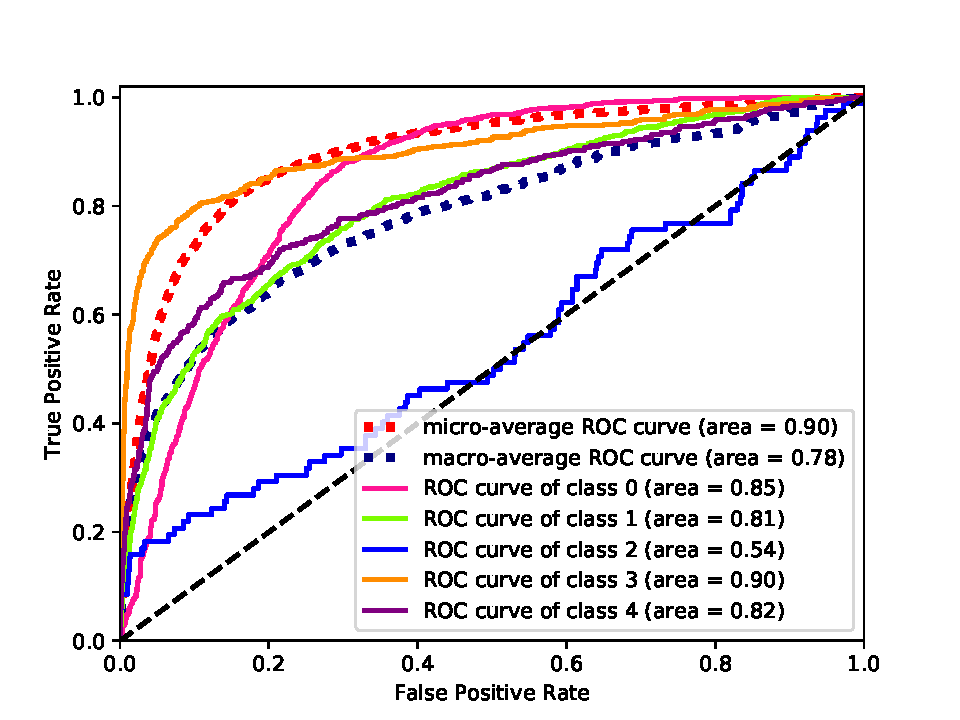
\includegraphics[width=6cm]{sections/figures/cnn_SUMTRIAN_100.pdf}\label{fig:auc_cnn_sum}}
  \hfill %\vspace{-0.4cm}
  \subfloat[]{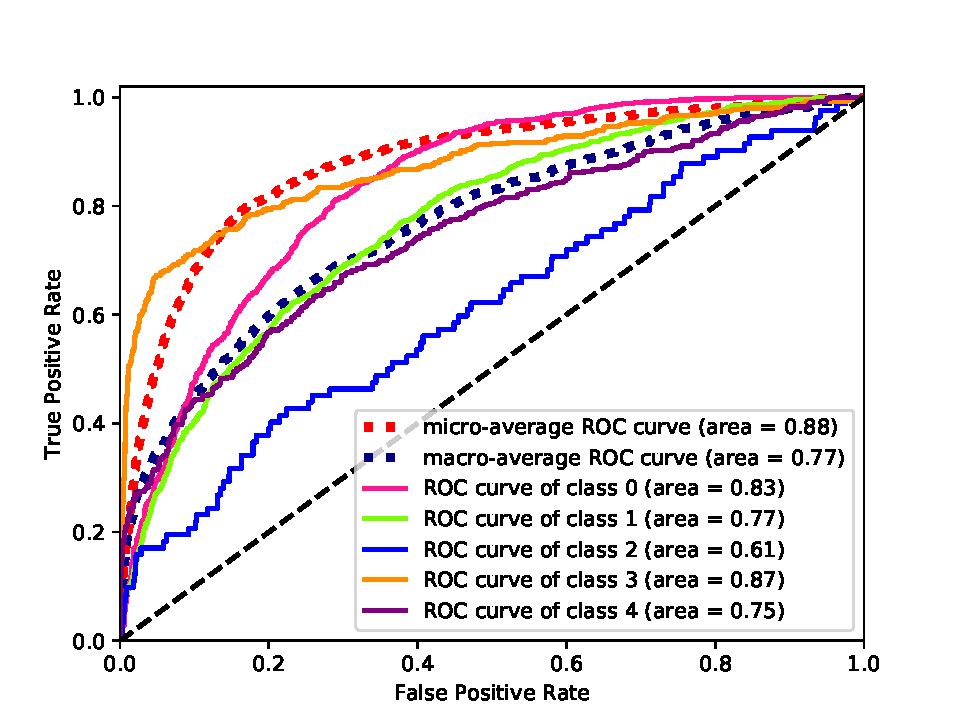
\includegraphics[width=6cm]{sections/figures/ae_cnn_multitask_SUMTRIAN_25.pdf}\label{fig:auc_ae_cnnmul_sum}}
  \caption{The ROC curves on the SUMTRIAN test set of the CNN trained with 100\% data (Fig.~\ref{fig:auc_cnn_sum}) and AE\_CNN\_Mul trained with 25\% data (Fig.~\ref{fig:auc_ae_cnnmul_sum}).}
 \label{fig:auc_sum}
\end{figure}

\begin{figure}[]
  \centering
%    \vfill %\vspace{-0.4cm}
  \subfloat[]{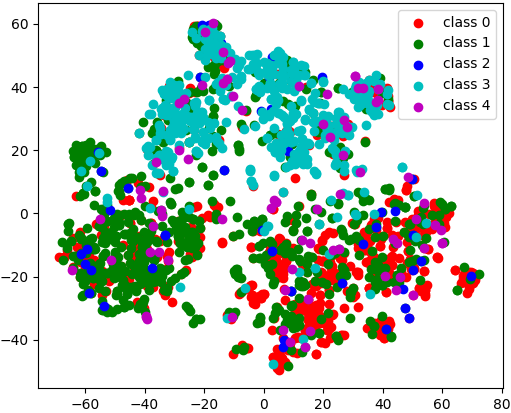
\includegraphics[width=6cm]{sections/figures/cnn_FLOW016_100_visualize.png}\label{fig:fea_cnn_flow}}
  \hfill %\vspace{-0.4cm}
  \subfloat[]{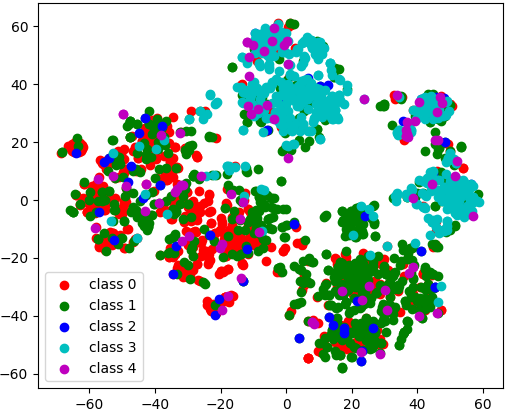
\includegraphics[width=6cm]{sections/figures/ae_cnn_FLOW016_100_visualize.png}\label{fig:fea_ae_cnn_flow}}
   \vfill %\vspace{-0.4cm}
    \subfloat[]{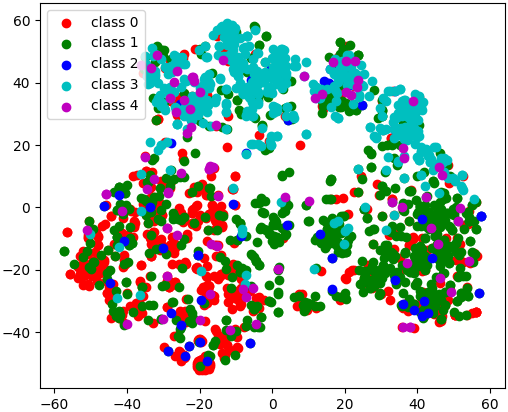
\includegraphics[width=6cm]{sections/figures/cnn_multi_task_FLOW016_100_visualize.png}\label{fig:fea_cnn_mul_flow}}
  \hfill %\vspace{-0.4cm}
  \subfloat[]{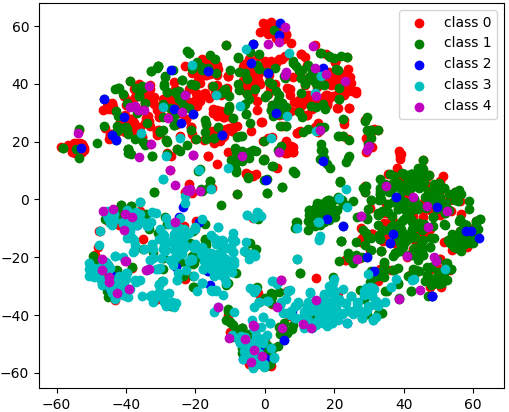
\includegraphics[width=6cm]{sections/figures/ae_cnn_multitask_FLOW016_100_visualize.png}\label{fig:fea_ae_cnn_mul_flow}}
  \caption{Feature visualization on the FLOW016 test set of methods CNN (Fig. \ref{fig:fea_cnn_flow}), AE\_CNN (Fig. \ref{fig:fea_cnn_flow}), CNN\_Mul (Fig. \ref{fig:fea_cnn_flow}), and AE\_CNN\_Mul (Fig. \ref{fig:fea_cnn_flow})}
 \label{fig:fea_flow016}
\end{figure}


\begin{figure}[]
  \centering
%    \vfill %\vspace{-0.4cm}
  \subfloat[]{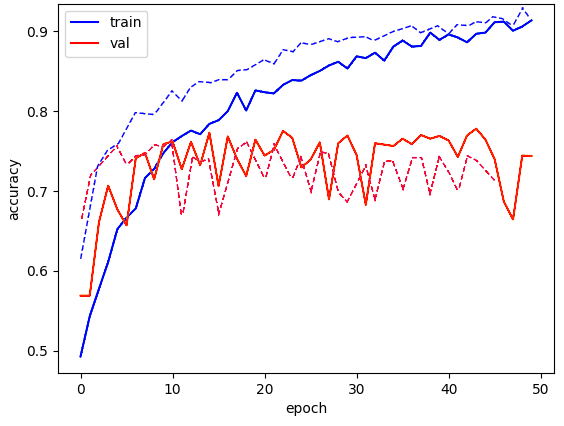
\includegraphics[width=6cm]{sections/figures/MNMX_25_train_valid_acc.png}\label{fig:mnmx_25_train_valid_acc}}
  \hfill %\vspace{-0.4cm}
  \subfloat[]{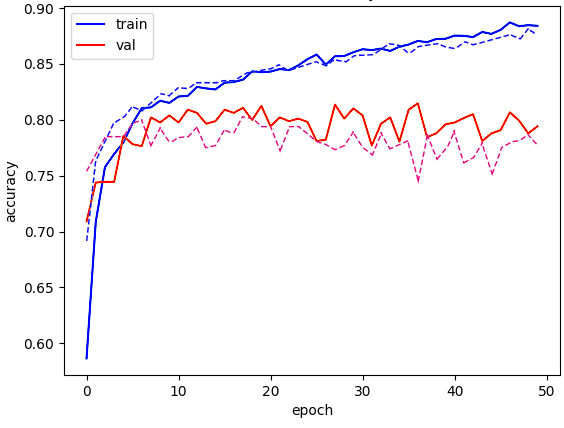
\includegraphics[width=6cm]{sections/figures/MNMX_100_train_valid_acc.png}\label{fig:mnmx_100_train_valid_acc}}
  \caption{The training process of AE\_CNN\_Mul (solid lines) and CNN\_Trans (dashed lines) classifiers on MNMX with 25\% (\ref{fig:mnmx_25_train_valid_acc}) and 100\% (\ref{fig:mnmx_100_train_valid_acc}) data.}
 \label{fig:mnmx_training_process}
\end{figure}